% \section{Outline}

% This essay is about computer simulations in healthcare and beyond. This all began from the following issues with our current system of evidence based medicine, as argued by Dr. Bernard Hsu in A future of medicine. 

% In this light, given the two aforementioned issues, Dr. Bernard proposes that computer simulations may render our current system of evidence based medicine irrelevant.

The following is about computer simulations in medicine and beyond. Motivated by the following arguments outlined by Dr. Bernard Hsu in A future of medicine.


\begin{enumerate}
    \item The first stems from human trials, where issues may arise if there is a disparity in efficacy, where one group may be effectively condemned to death.\textsuperscript{(Harmon)}
     
    \item The second pertains to issues in generalizing data from human trials for predicting outcome for a given individual. For instance, as Dr. Bernard points out, if a trial was done on a bunch of men, clinical experience suggests that there will be differences for women taking the same medication.\textsuperscript{(Bernard)}''. 
\end{enumerate}

Nowadays, trials are required to include notable age, gender, and race/ethnicity demographics. But as Kravitz pointed out, ``[this] may do nothing but ensure that the estimates for any one subgroup are unreliable due to small numbers''. In the very same paper, Kravitz coined this phenomena, the ``Heterogeneity of Treatment Effects. 

To further illustrate the utility of what I am proposing, consider the following thought experiment. What if, instead of running a trial on thousands of disperse persons. What if you were simply cloned, hundreds of thousands of times, and therein, we performed hundreds of thousands of trials, forming a model that likewise predicts outcome for some given treatment?

But, you may be asking, how exactly do we run hundreds of thousands of trials of my identical clones? We run computer simulations, as Dr. Bernard proposed. Although what Dr. Bernard proposed, was essentially a thought experiment, explicitly regarding this as something that probably won't be viable in our lifetime. Conversely, my research paper will say otherwise.

% From personal experience, it seems as though technological innovation occurs in an incremental and continuous fashion. That is, there is never some removable jump discontinuity in the graph of progress. On this grounds, presumably we will see smaller increments of Dr. Bernard's hypothetical system.



% Working backwards, before we see whole person simulations, we may see more targeted usage of such. The current director of the Hugh Kaul Precision Medicine Institute is helmed, not by a medical doctor, but by a Ph.D. in Computer Science. His story begins with his son, who was born with a rare genetic disorder that had no known treatments. Essentially, he used computation to discover pathways (presumably using open biological databases) that work around a malformed protein. As he put it, in essence, if red increases green, and green decreases blue, then we can decrease blue by increasing red. In this case, he used the Kappa programming language and constructed a model based on a series of constraints that the computer must satisfy. It's regarded as an old form of machine learning, and unlike modern machine learning, the solution isn’t ‘inferred’. As in, ‘how’ it arrives at a given answer will be known.

% Why this is relevant to my talk is because this resembles what we may perhaps consider to be the forerunner to Dr. Bernard's hypothetical replacement to our current standard of evidence based medicine that is founded on computer modeling, and furthermore, this essentially means that there will be a market for incremental developments in computer modeling and simulation technologies. Because ultimately, Dr. Bernard's hypothetical system will have to be accepted by the preexisting medical establishment, bridges that Matt Might and the greater precision medicine movement may be creating. 

% \section{Simulations}
\section*{Realization}

In his TED-X talk, Rahul Sarpeshkar discussed the prospects of analog computing in the context of biological processes and electronic analog hardware. Therein, Sarpeshkar claimed that we could viably simulate an entire person if we built an analog computer that spanned the size of the given auditorium.

This is due, not to processing performance, but as Sarpeshkar argues, in information theory. That is, digital computation in contrast, while built upon analog mediums, forgoes most of the real estate therein for a limited set of gates defined in terms of a mere bit, in a single multi-bit analog channel. Conversely, in allowing full utilization of the unclaimed and unexploited real estate therefrom, in further expanding our conception of computation to more than mere logic, new applications may potentially become commercially viable. Such as perhaps, simulating the molecular interactions within cells, to tissues, to entire organ systems, to perhaps, entire persons. Or rather, as Sarpeshkar summarized:

\begin{quotation}
    [at] low informational precision, logic basis functions simply cannot compete with the richer basis functions of analog computation that can process all the bits at once in parallel and just automatically solve the task, e.g. by using Kirchoff’s current law for addition or chemical binding for multiplication.\textsuperscript{(Sarpeshkar)}
\end{quotation}


% So to summarize, what Dr. Bernard proposed, was essentially a thought experiment, explicitly regarding this as something that probably won't be viable in our lifetime. Conversely, my research paper will say otherwise, by forgoing a multitude of modern innovations, from the von-neumann architecture, digital computer architectures, numerical precision, and ultimately, generality. In favor of analog computer architectures that more directly models the natural phenomena it's tasked with simulating.  Notably, analog computing more efficiency solves the differential equations governing the various processes taking place within your body, in a manner that conventional computer architectures are fundamentally ill adept at. Which, in this respect, Sarpeshkar argues that analog computing is more efficient in terms of energy, time (computation) and space (memory and program installation).

To explain why, imagine we somehow needed to compute one instruction for each atom, for each cell, in the human body. Which would then amount to $4 \mathrm{x} 10^{27}$ instructions. To imagine this in terms of time. Consider first, simply the latency overhead incurred when your processing hardware and main memory is physically separated from each other, and therefore, each instruction must first read some datum from main memory. Lets say this overhead is $100\mathrm{ns}$ per instruction. Then latency overhead alone will amount to $4\;\mathrm{x}\;10^{20}$ seconds, or in other words, latency overhead alone will total $12,683,916,800,000$ years per evolution. But obviously, you may be saying, we can reduce runtime in parallelizing work.

Instead we may turn our attention to super computers. Considering for instance, Tianhe-1A: initial costs amounted to $\$88$ million dollars, and another $\$20$ million dollars is spent, per year, on power consumption.\textsuperscript{(Tianhe-1)} This means that after four years, power consumption alone become the most significant cost factor. In contrast, Trafton argues that, ``[in] one second, a [typical] cell performs about 10 million energy-consuming chemical reactions, which altogether require about one picowatt (one millionth millionth of a watt) of power.''\textsuperscript{(Trafton)} Even for one of the more power hungry human organs (relative to weight), the human brain, requires a mere 12 to 15 watts of power, to sustain trillions of operations therein. (Which is about the power consumption of a lightbulb.) The energy efficiency therefrom, as Sarpeshkar proposes, is again, the product of forgoing high precision operations in favor of low precision analog computation with feedback mechanisms.

% (Sarpeshkar and Teo have argued that the power efficiency of cells, stems from forgoing precision to the maxim possible extent that the operations therein affords. Which as Teo argues, pushes cells ``near the thermodynamic limits of physics''.)


\section*{\raggedright Analog Computers}

Digital computation is discreet, and proceeds in terms of discrete steps. All representations in digital form, are mere, and meaningless symbols. Computer arithmetic for instance, is simply the manipulation of such symbols is manner that implements such operations. This is also, the greatest strength to discrete computation. Remember those pen n' paper procedures you were taught for adding arbitrary numbers together? Digital computation implements the very same processes, and so, can scale to adding arbitrary numbers without loss of precision\textsuperscript{(Hehner)}.

Conversely, the central issue plaguing analog computers is that of precision, typically bounded to just three or four bits. Yet, advocates of analog computers argue that many problems do not exceed such limitations, and therefore permits implementation in an analog environment that affords a greater degree of optimizations that aren't possible on digital computer architectures. In a similar manner, MacLennan adds that analog environments are a natural fit for noisy and low resolution real world measurements.\textsuperscript{(MacLennan)}

% Likewise, Sarpeshkar argues that the fundamental limitations of analog computing, notably, noisy signals, is ideal for simulating stochastic process. Because simulating randomness on digital hardware imposes synchronization constraints that significantly impacts performance on such systems. Whereas on analog architectures, Sarpeshkar argues, you essentially get such for free.

% Therefore, overall, while discrete computer architectures are incredibly versatile, such may not necessarily be efficient. Furthermore when it comes to solving, say, differential equations, analog computing is unrivaled. Consider, for instance, the following digram that implements $\ddot{y} = -y$. 

\ifpdf
  FIGURE
\else
  \begin{figure}[H]
    \centering
    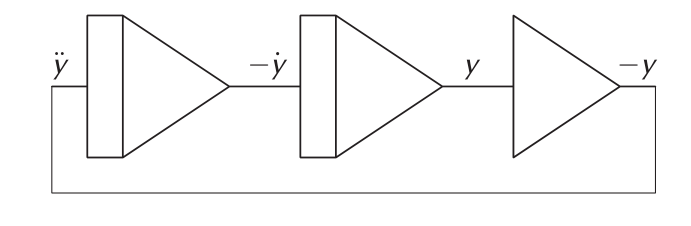
\includegraphics[width=0.7\linewidth,natwidth=500,natheight=200]{../assets/analogue-computing-fun-differential-equations.png}
    \caption{\bibent
    Source: \url{https://chalkdustmagazine.com/features/analogue-computing-fun-differential-equations/}. (Note that this is missing initial conditions.)}
    \label{Image Label}
\end{figure}
\fi

In the above figure, the leftmost elements are the integrators, while the rightmost element is called the summer, and each elements implicitly flips the sign. Personally, there is an elegant economy to the above diagram, and furthermore, it implements such without requiring stored computer memory, and this itself is notable (as I will try to explain shortly). In contrast, implementing the same processes on digital computer architectures would require significantly more infrastructure in implementing the same mathematical laws in terms of manipulations of arbitrary symbols. Which obviously increases overall costs, size, energy requirements, and so forth.

As MacLennan wrote, in digital computation, quantities are rather arbitrary symbols that have no direct relationship to the physical systems that such may be tasked with simulating. In contrast, generally speaking, analog and physical phenomena are governed and defined by the same mathematical laws. Or as MacLennan put it, ``the computational quantities are proportional to the modeled quantities.''

% Although my aforementioned analog may be a ludicrous exercise, because for instance, what is meant by one instruction per atom? But crucially, remember the aforementioned digram that implements $\ddot{y} = -y$? Such problems needn't concern such implementations.

\section*{Compatibility}

Some authors have argued that there is, as I have put it, an isomorphism between chemistry and electric analog circuitry. Two things are isomorphic if we can define a mapping between such objects without loss of information, which resembles the relationship proposes by Teo, as argued,
\begin{quotation}
    There is a deep connection between ‘electronics’, which is about the controlled, relatively long-range motions of electrons between devices, and ‘chemistry’, which is about the controlled, relatively short-range motions of electrons between atoms and molecules.\textsuperscript{(Teo)}
\end{quotation}

That is, we have a model that can manifest in chemical systems and electric analog circuitry, from this link between electronics (simulation) and chemistry (e.g. biochemical computation). Alternatively, as Sarpeshkar wrote,
\begin{quotation}
    There are striking similarities between chemical-reaction dynamics (figure 3a) and electronic current flow in the subthreshold regime of transistor operation (figure 3b): electron concentration at the source is analogous to reactant concentration; electron concentration at the drain is analogous to product concentration; forward and reverse current flows in the transistor are analogous to forward and reverse reaction rates in a chemical reaction; the forward and reverse currents in a transistor are exponential in voltage differences at its terminals analogous to reaction rates being exponential in the free-energy differences in a chemical reaction; increases in gate voltage lower energy barriers in a transistor increasing current flow analogous to the effects of enzymes or catalysts in chemical reactions that increase reaction rates; and the stochastics of the Poisson shot noise in subthreshold transistors are analogous to the stochastics of molecular shot noise in reactions. [...] The logarithmic dependence of the electrochemical potential in chemical concentration or of current enables one to map log-domain analog transistor circuit motifs in electronics to log-domain analog molecular circuit motifs in cells and vice versa.\textsuperscript{(Sarpeshkar)}
\end{quotation}

% Therefore, we have a means of translating the computation that manifests in chemical systems, to electronic analog computers where such systems may be redefined, and furthermore, abstracted. In a manner akin to the aspirations from the field of synthetic biology, which attempts to unify engineering principles with biology.

% In this intersection, we have a foundation that reduces biology to software. With a proper software ecosystem in place, these bottom-up, cumulative processes may give rise to very sophisticated products, and perhaps one day, akin to the emergent phenomena seen in nature itself.

Therefore, we have a means of translating the computation that manifests in chemical systems, to electronic analog computers where such systems may be redefined, and furthermore, abstracted. In this intersection, we have a foundation that reduces biology to software. With a proper software ecosystem in place, these bottom-up, cumulative processes may give rise to very sophisticated products, and perhaps one day, akin to the emergent phenomena seen in nature itself, as I will explain in the following section. 

\section*{\raggedright What Affordability Offers}

% Why this is important is because, even an approximation of the best case scenario leads to a platform that favors experimentation and iteration, by both small and underfunded terms, to billion dollar pharmaceutical companies.

% Which I argue, has far reaching implications. Because

% If we can reduce natural 

% this reduces modeling to programming, and from programming, abstraction. Why does this matter?

% For a multitude of reasons. First, humans are utterly unrivaled when it comes to natures ability to self assemble into sophisticated structures (including ourselves).

I believe that accessibility benefits everyone, just as much as I believe that reducing the barrier to entry in engineering disciplines, results in more innovation, and more sophisticated products therefrom. In this regard, software is perhaps the most accessible, because you don't need a lab stocked with expensive ad hoc equipment. But in this case, perhaps, access to some cloud based compute infrastructure that affords easy and cheap access to the more specialized analog computing hardware.

Furthermore, humans are utterly unrivaled when it comes to natures ability to self assemble into sophisticated structures (including ourselves). That is, we can plant a seed, and grow a tree, but planting a seed to grow a house is unfathomable. Just as unfathomable as designing robots to kill cancer cells, which again, nature has parallels.  Presumably this is due to complex factors that may be abstracted within my proposed computer architecture. (Remember that aforementioned isomorphism?)

When we abstract, we may sometimes reduce `complex' things into simpler, more conceptually `discrete' things. Which therein, due to this simpler nature, may further permit others to effectively build upon such, and therein, may create something more sophisticated, perhaps even, greater than the sum of it's components. 

That is, a system where discrete units build upon other discrete units and therein produce more complex non-discrete units. This system permits for abstraction, so complex non-discrete units may be abstracted into simple discrete units. Thereafter this process of production and abstraction enables further production and abstraction and so forth. Each iteration or generation may be considered to be more sophisticated than prior generations, given that each generation is a product of prior generations… From this analogy, you can imagine these bottom-up and cumulative processes will eventually give rise to very sophisticated products, and perhaps one day, akin to how emergence gives rise to the complexity found in nature.

From personal experience, my \url{https://imager.io} project wouldn’t be possible without the various open source components it’s built upon. Simply because my time is finite, and especially because lower-level encoding details are just \textbf{too complicated for me to understand and implement on my own}. I am nevertheless able to compose such components into a larger and more sophisticated end product.

% In this manner, to me, abstraction is akin to a force multiplier of the human mind.

% , from the preexisting output of resources and information from the global open source, software community. Overall added value that may be considered to be greater than the sum of its components, and therefore emergent in a manner of speaking. In an old English paper I likened the open source community as ``the printing press of computable knowledge'', and perhaps even more significant than the advent of the printing press itself, because as the industrial revolution introduced a force multiplier of human muscle, so too does abstraction introduce a force multiplier of the human mind.

% Because, while a book may describe a life’s work in mathematics and applications therein, the medium is itself rather passive. A book may describe a life’s work in applied mathematics, yet a mind is required to manifest its application. Whereas, imagine a medium where the most knowledgeable of experts can record their understanding of a given domain as functions that map problems to solutions, in a manner that can be utilized by any layperson, and thereafter this record can be reapplied, reused, and so forth, forever thereafter, and, in this manner, what are the ramifications of such?

% Furthermore, if you can build upon abstracted systems written by experts, where these abstractions mask complexity, we may then presume that the overall barrier to entry will drop. That is again, if laypersons are able to built upon abstracted systems in a manner that doesn't require an expert understanding or formal education in such (and presumably in a manner akin to my aforementioned \url{https://imager.io} story). But on the other end, if the barrier to entry is lower, this implies reduced costs, and therefore, we may likewise see significant cost savings in industries built upon such, perhaps in a manner akin to using ``higher level'' programming languages for applicable problems. 

Just as the industrial revolution introduced a force multiplier of human muscle, so too does abstraction introduce a force multiplier of the human mind. What we need now, as I have argued, is a paradigm shift in amplifying our ability to rival the sophistication we see in nature. 

